\documentclass[a4paper,11pt]{article}
\usepackage[english]{babel}
\usepackage[utf8]{inputenc}
\usepackage{amsmath,amsfonts,amsthm,amssymb,tikz}
\usetikzlibrary{arrows}
\usetikzlibrary{shapes}
\usepackage{contmech}
\begin{document}
\centering


\begin{figure}
%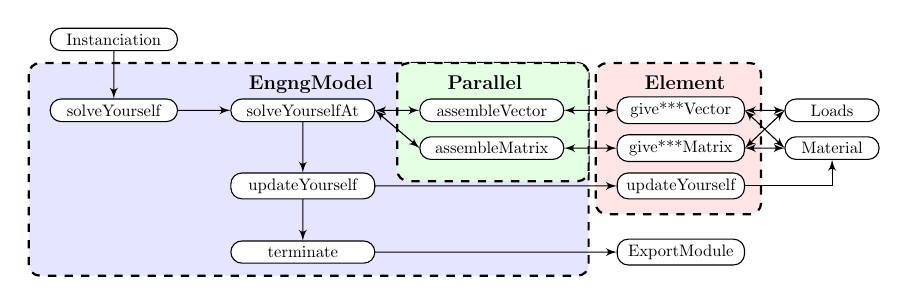
\begin{tikzpicture}[node distance = 2cm, auto,scale=0.6, transform shape]
    %\small
    %\tikzstyle{every node}=[font=\footnotesize]
    \tikzstyle{group}    = [rectangle, draw, thick, dashed, text width=6em, text centered, rounded corners]
    \tikzstyle{decision} = [diamond,   draw, fill=white, text width=6em, text centered, node distance=2.5cm, inner sep=0pt]
    \tikzstyle{block}    = [rectangle, draw, fill=white, text width=6em, text centered, rounded corners]
    \tikzstyle{line}     = [draw, -latex']

    \draw [thick, dashed, fill=blue!10, rounded corners] (-1.8,-0.5) rectangle (10.05,-5);
    \draw [thick, dashed, fill=red!10,  rounded corners] (10.2,-0.5) rectangle (13.7,-3.7);
    \draw [thick, dashed, fill=green!10,  rounded corners] (6.0,-0.5) rectangle (10.05,-3.0);
    \node [below right, inner sep=10pt] at (2.5,-0.4) { \textbf{\large EngngModel} };
    \node [below left,  inner sep=10pt] at (13.3,-0.4) { \textbf{\large Element} };
    \node [below left,  inner sep=10pt] at (9.0,-0.4) { \textbf{\large Parallel} };

    % Place nodes
    % Engineering model:
    \node [block, text width=7em] (init) {Instanciation};
    \node [block, below of=init, text width=7em, node distance=1.5cm] (solve) {solveYourself};
    \node [block, right of=solve, text width=8em, node distance=4.0cm] (solveAt) {solveYourselfAt};
    \node [block, right of=solveAt, text width=8em, node distance=4.0cm] (assembleVector) {assembleVector};
    \node [block, below of=assembleVector, text width=8em, node distance=0.8cm] (assembleMatrix) {assembleMatrix};
    \node [block, below of=solveAt, text width=8em, node distance=1.6cm] (update) {updateYourself};
    \node [block, below of=update, text width=8em, node distance=1.4cm] (terminate) {terminate};

   % Element
   \node [block, right of=assembleVector, text width=7em, node distance=4.0cm] (giveVector) {give***Vector};
   \node [block, right of=assembleMatrix, text width=7em, node distance=4.0cm] (giveMatrix) {give***Matrix};
   \node [block, below of=giveMatrix, text width=7em, node distance=0.8cm] (elementUpdate) {updateYourself};

   % Other
   \node [block, right of=giveVector, text width=5em, node distance=3.2cm] (loads) {Loads};
   \node [block, right of=giveMatrix, text width=5em, node distance=3.2cm] (material) {Material};
   \node [block, below of=elementUpdate, text width=7em, node distance=1.4cm] (export) {ExportModule};


   \path [line] (init) -- (solve);
   \path [line] (solve) -- (solveAt);
   \path [line] (solveAt) -- (update);
   \path [line] (update) -- (terminate);
   \path [line] (terminate) -- (export);
   \path [line,latex'-latex'] (solveAt.east) -- (assembleVector.west);
   \path [line,latex'-latex'] (solveAt.east) -- (assembleMatrix.west);
   \path [line,latex'-latex'] (assembleVector) -- (giveVector);
   \path [line,latex'-latex'] (assembleMatrix) -- (giveMatrix);

   \path [line,-latex'] (update.east) -- (elementUpdate.west);
   \path [line,latex'-latex'] (giveVector.east) -- (material.west);
   \path [line,latex'-latex'] (giveVector.east) -- (loads.west);
   \path [line,latex'-latex'] (giveMatrix.east) -- (material.west);
   \path [line,latex'-latex'] (giveMatrix.east) -- (loads.west);

   \path [line,-latex'] (elementUpdate.east) -| (material.south);
\end{tikzpicture}
%h = rand(2)*0.5; hsym = 0.5*(h + h'); hsymdev = hsym - mean(diag(hsym))*eye(2);
%u1 = h*c; u2 = hsymdev*c; c1 = c+u1; c2 = c+u2;
%all = [1:4,1]
%plot(c(1,all), c(2,all), '--', c1(1,all), c1(2,all), 'b-', c2(1,all), c2(2,all), 'r-')
%printf("(%f, %f) -- ", c1(:,all))
%printf("(%f, %f) -- ", c2(:,all))

\begin{tikzpicture}[]
 \node (D) at (0,2.5) {$\bar{\ta u}, \bar{\ts h}, \bar p$};
 \draw[densely dashed] (-0.5,-0.5) rectangle (0.5,0.5);
 \draw[] (-0.679901, -0.785203) -- (0.562857, -0.370962) -- (0.679901, 0.785203) -- (-0.562857, 0.370962) -- (-0.679901, -0.785203);
 \node at (3,0) {$\begin{cases} \bar{\ts\sigma}_\dev\{\bar{\ts h}_\dev^\sym, \bar{p}\} \\ \bar{e}\{\bar{\ts h}_\dev^\sym, \bar{p}\}\end{cases}$};
 \draw[->] (D.south) -- +(0,-1.5);
 \draw[->] (D.south) -- +(0,-1.5);
 \draw[->] (0.7,0) -- (1.4,0);

 \begin{scope}[shift={(6,0)}]
 \draw[densely dashed] (-0.5,-0.5) rectangle (0.5,0.5);
 \draw[] (-0.654469, -0.611173) -- (0.388827, -0.345531) -- (0.654469, 0.611173) -- (-0.388827, 0.345531) -- (-0.654469, -0.611173);
 \node (A) at (0,2.5) {$\bar{\ta u}, \bar{\ts h}, \bar p$};
 \node (B) at (0,1.5) {$\bar{\ts \epsilon}_\dev = \bar{\ts h}_\dev^\sym, \bar{p}$};
 \node[anchor=west] at (1.5,1.5) {($\bar{\ts h}^\skw, \bar{h}_\vol, \bar{\ta u}$ are void)};
 \node at (3,0) {$\begin{cases} \bar{\ts\sigma}_\dev\{\bar{\ts\epsilon}_\dev, \bar{p}\} \\ \bar{e}\{\bar{\ts\epsilon}_\dev, \bar{p}\}\end{cases}$};
 \draw[->] (A.south) -- (B.north);
 \draw[->] (B.south) -- +(0,-0.5);
 \draw[->] (0.7,0) -- (1.4,0);
 \end{scope}
 
\end{tikzpicture}
\end{figure}
\end{document}